\chapter{Opis projektnog zadatka}
	
Cilj ovog projekta je razvoj aplikacije FlipMemo u svrhu učenja riječi na stranom jeziku. 
FlipMemo je namijenjen svima koji žele unaprijediti svoje znanje na interaktivan i efikasan način. 
Aplikacija omogućuje početnicima kao i naprednim korisnicima razvijanje svoje vještine razumijevanja, 
čitanja i pisanja stranog jezika. Učenje se oslanja na tehniku ponavljanja s rastućim vremenskim razmacima. 
Aplikaciju će moći koristiti bilo tko zainteresiran za učenje jezika, te sve što je potrebno je adresa elektroničke pošte.

\section{Ponavljanje s rastućim vremenskim razmakom}

SR (iz engleskog „spaced repetition”) tehnika je napravljena tako da iskoristi psihološki efekt prisjećanja. 
Naime, ljudi prirodno zaboravljaju informacije koje ne koriste često, jer ljudska memorija nije beskonačna, 
pa stvari koje nisu dio svakodnevice postaju dio zaborava. Ta činjenica još više vrijedi za nove informacije. 
Informacija koju ne koristimo ili ne vežemo s iskustvom se jednostavno ne smatra važnom, stoga se lako zaboravi. 
SR tehnika rješava ovaj problem tako što informacije koje želimo naučiti (u našem slučaju riječi jezika) pretvara u dio svakodnevice.

\begin{figure}[H]
	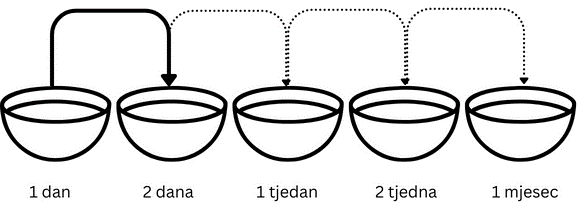
\includegraphics[scale=0.8]{slike/spaced_repetition.png} 
	\centering
	\caption{Ilustracija sustava za učenje s pet posuda}
	\label{fig:spacedrepetition}
\end{figure}

Kako bismo lakše razumjeli ovaj način učenja, zamislimo nekoliko posuda, kao na slici \ref{fig:spacedrepetition}. 
U svakoj posudi se nalaze kartice s informacijama koje korisnik želi naučiti. Na karticama se nalazi pitanje i odgovor. 
Svaka posuda je označena sa svojim vremenskim intervalom. Svaka kartica na koju se da točan odgovor ide u sljedeću posudu.
 Svaka kartica na koju se da netočan odgovor, ide u prvu posudu. Ako se na karticu odgovori točno, a bila je izvađena iz zadnje 
 posude, kartica izlazi iz sistema i ta informacija se smatra naučenom. Korisnik na početku sesije učenja vadi sve kartice iz prve 
 posude, te odgovara na pitanja. One na koje odgovori točno, stavlja u posudu od dva dana, one na koje odgovori netočno, ostavlja u 
 posudu od jednog dana. Kad završi sa svim pitanjima, sesija je za taj dan gotova. Ako korisnik odluči učiti odmah dan nakon, može vaditi 
 kartice iz prve posude, ali ne iz druge. Tek nakon prolaska dva dana može opet uzeti kartice iz druge posude.

Cilj je u tome da se informacije koje teže ili manje pamte, viđaju češće. Stvari koje korisnik zna ili razumije lakše, viđa manje, čime se može fokusirati na nedostatke u svom znanju.

\eject
\section{Opis aplikacije}

Aplikacija je kolekcija rječnika iz kojih se mogu učiti riječi odabranog jezika. Rječnik je kolekcija međusobno značenjem povezanih riječi. 
Svaka riječ ima svoj prijevod na hrvatski, te prijevode na implementirane strane jezike, značenje tih riječi, pomoćne rečenice unutar kojih se 
ta riječ koristi i audiozapis izgovora riječi na svakom od njih. Riječi dodaju administratori riječi, čije ovlasti može dati jedan korijenski administrator. 
Korisnici imaju pristup svim rječnicima odabranog jezika za učenje, te četiri načina učenja.

Riječi i rječnici su odgovornost administratora riječi. Pri dodavanju riječi u sustav, administrator je dužan pobrinuti se za točnost 
prijevoda i značenja, kao i pomoćne rečenice i audiozapisa izgovora riječi. U tom poslu mu pomaže API. Jednu riječ može dijeliti više rječnika. 

Dizajn aplikacije je fokusiran na intuitivnost i jednostavnost. Cilj je napraviti proizvod koji ne pruža prilike
za pogrešno korištenje, te korisnicima pruža sigurnu i efikasnu uslugu. Korisničko sučelje se razlikuje
ovisno o vrsti prijavljenog korisnika. Administratorsko sučelje pruža isključivo funkcionalnosti izmjene i dorađivanja
riječi i rječnika, dok učeničko sučelje ima samo pristup opcijama vezanima za učenje. Svi vizualni elementi se
oslanjaju na minimalnost i responzivnost.

\subsection{Načini učenja} 

U aplikaciji su predviđena četiri načina učenja, kako bi savladavanje gradiva išlo što lakše i brže:
\begin{description}
	\item[Foreign prompt --- native translation:] Korisniku je prikazana riječ stranog jezika. Ponuđeno mu je nekoliko riječi na hrvatskom jeziku od 
	kojih on mora odabrati onu koja je najbolji prijevod strane riječi. Riječi koje se nude kao odgovori biraju se iz trenutno aktivnog rječnika, tj. rječnika iz kojeg se uči. 

	\item[Native translation --- foreign prompt:] Korisniku je prikazana riječ na hrvatskom jeziku, te mu je ponuđeno nekoliko riječi na stranom jeziku. 
	Korisnik od njih mora odabrati onu koja je točan prijevod riječi na hrvatskom jeziku.

	\item[Listen and translate:] Korisnik sluša audiozapis izgovora trenutne riječi na odabranom jeziku učenja. Korisnik treba napisati 
	riječ koju je čuo. Time se provjerava razumije li korisnik razlike u izgovoru riječi kao i njihovo pisanje.

	\item[Record your translation:] Korisnik dobiva riječ na jeziku koji uči i opciju za snimanje glasa. Potrebno je točno 
	izgovoriti riječ prikazanu na ekranu. Ocjena izgovora može biti brojka od jedan do deset, čime korisnik dobiva povratnu informaciju o svom izgovoru.
\end{description}

Nakon svakog odgovorenog pitanja, korisnik dobiva povratnu informaciju o točnosti odgovora. Kad korisnik završi sa 
sesijom učenja i prođe sve riječi za taj dan aplikacija mu javlja da je za taj dan s tim rječnikom gotov. 

\eject

\section{Slična rješenja i tržište}

Kao što je već spomenuto, aplikaciju može koristiti bilo tko ima email adresu. Može biti korisna učenicima u školama, 
kao sredstvo za samostalni rad, ali mogu je i sami nastavnici preporučivati ili čak integrirati u nastavu. Aplikacija također može biti 
korisna predanim turistima koji se spremaju za putovanje u državu u kojoj ne poznaju jezik, ili čak poslovnim ljudima koji imaju čest dodir 
sa stranim kulturama u svakodnevici. 

Konkurenciju nam predstavlja Anki, aplikacija koja je agnostična na informacije koje se proučavaju. Korisnici mogu samostalno 
napraviti kolekcije kartica za učenje i dijeliti ih međusobno. S jedne strane, to je dobra stvar, jer se može učiti bilo koja tema koja 
se poželi, no s druge strane, ako korisnik nije voljan ili nema vremena praviti kartice za učenje, a netko nije napravio kvalitetnu kolekciju i 
ponudio ostalim korisnicima, taj korisnik ne može učiti. Specijalizacija naše aplikacije na jezike osigurava kvalitetu učenja i kvalitetu kartica.

\begin{figure}[H]
	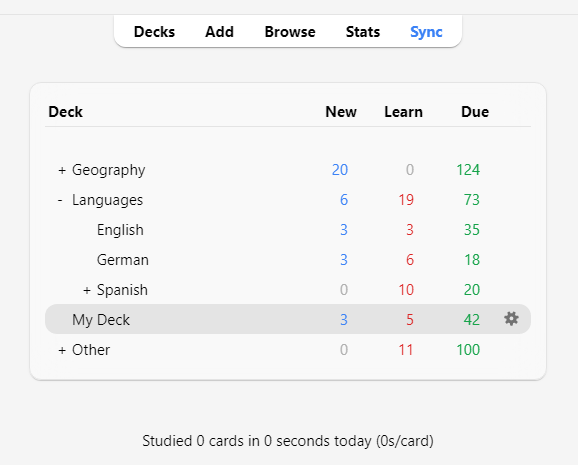
\includegraphics[scale=0.8]{slike/anki_screen.png} 
	\centering
	\caption{Špilovi u Ankiju pandan su našim rječnicima}
	\label{fig:ankideck}
\end{figure}

\eject